\documentclass{article}
\usepackage{tikz}
\usetikzlibrary{positioning}
\begin{document}
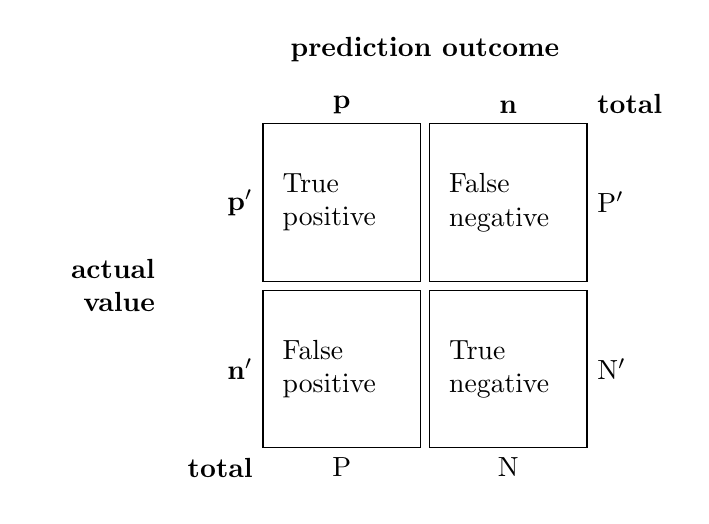
\begin{tikzpicture}[
box/.style={draw,rectangle,minimum size=2cm,text width=1.5cm,align=left}]
\matrix (conmat) [row sep=.1cm,column sep=.1cm] {
\node (tpos) [box,
    label=left:\( \mathbf{p'} \),
    label=above:\( \mathbf{p} \),
    ] {True \\ positive};
&
\node (fneg) [box,
    label=above:\textbf{n},
    label=above right:\textbf{total},
    label=right:\( \mathrm{P}' \)] {False \\ negative};
\\
\node (fpos) [box,
    label=left:\( \mathbf{n'} \),
    label=below left:\textbf{total},
    label=below:P] {False \\ positive};
&
\node (tneg) [box,
    label=right:\( \mathrm{N}' \),
    label=below:N] {True \\ negative};
\\
};
\node [left=.05cm of conmat,text width=1.5cm,align=right] {\textbf{actual \\ value}};
\node [above=.05cm of conmat] {\textbf{prediction outcome}};
\end{tikzpicture}
\end{document}